\chapter{PCG for Threshold BBS+}
\label{chapter:PCGforBBSPlus}
In this chapter, we recall and evaluate an application for PCGs in regard to realizing a threshold signature scheme (cf. Definition \ref{def:tss}) based on BBS+ (cf. Construction \ref{definition:bbs+}). Recent threshold BBS+ schemes \cite{gennaro2019fully, doerner2023threshold} necessitate interaction among parties during signing, resulting in communication overhead that leads to latency, especially in scenarios where the signing parties are geographically dispersed. Faust et al. \cite{faust2023non} address this limitation with a threshold BBS+ scheme that strategically divides the signing process into two phases: an interactive \textit{offline} preprocessing phase generating message-independent presignatures and a non-interactive \textit{online} signing phase where presignatures are used without further communication between signers. Besides achieving sublinear communication complexity in the offline phase, the essential advantage of this approach is the trade-off it offers. Shifting computationally demanding operations to the offline phase enables a highly efficient online signing process. This flexibility is beneficial for real-world applications that deal with variable utilization patterns and/or geographically dispersed parties, allowing presignature generation during low-demand periods to then enable rapid signature creation during peak system load. 
\\\\
We begin by recalling the threshold BBS+ scheme by Faust et al. \cite{faust2023non}. We explain how the scheme thresholdizes standard BBS+ to achieve applicability of PCGs, such that their expansion enables the offline preprocessing phase. Then, we present a complete construction for the $n$-out-of-$n$ case based on the PCG for (V)OLE from Section \ref{sec:construction}. Further, we show the necessary adaptions to realize the threshold $t$-out-of-$n$ case. Finally, we implement both cases, provide benchmarks to evaluate the construction, and derive implications for the efficiency of the online phase. 

\section{Thresholdization}
Refer to Construction \ref{definition:bbs+} for the standard BBS+ signature scheme. For simplicity, we focus on the $n$-out-of-$n$ scenario. Therefore, the key generation (\texttt{\textup{KeyGen}}) can be distributed via additive secret sharing. For an $t$-out-of-$n$ scenario, Shamir's Secret Sharing  \cite{shamir1979share} (which employs Lagrange interpolation) would be utilized. Notice that for adapting the signing (\texttt{\textup{Sign}}), the main difficulty lies in distributing the computation of Equation \ref{eq:BBS+standardA}.

\begin{equation}
A := \left( g_1\cdot h_0^s\cdot \prod_{\ell \in [k]} h_{\ell}^{m_{\ell}} \right)^{\frac{1}{x+e}}.
\label{eq:BBS+standardA}
\end{equation}

For realizing the non-interactive online phase, the thresholdization must be able to create message-independent presignatures for $A$ while preventing the disclosure of the secret key (shares of) $x$ during the computation of the inverse of $(x+e)$. This challenge is similar to those faced in other signature schemes that depend on exponentiation, such as ECDSA. Commonly, solving this involves calculating and revealing a value $B = M^a$ and $\delta = a\cdot x$ for a randomly chosen blinding value $a$. The signature of the massage $M^{1/x}$ can then be computed through $B$ without revealing $x$, since $M^{1/x} = B^{1/\delta}$. This is suitable for message-independent presignatures, as $\delta$ remains independent of $M$. This idea is applied in the following:
\\\\
\textbf{BBS+ presignature tuples.} For a $n$-out-of-$n$ setting, secret key $x$ and random blinding factor $a$, we define a BBS+ presignature $\varphi_i$ held by party $P_i$ as a tuple $(a_i,e_i,s_i,\delta_i,\alpha_i) \in \mathbb{Z}^5_q$, such that the following correlations hold

\begin{equation}
\begin{array}{l}
\delta=\sum\limits_{i \in[n]} \delta_i=a(x+e), \quad
\sum\limits_{i \in[n]} \alpha_i=as, \\
a=\sum\limits_{i \in[n]} a_i, \quad e=\sum\limits_{i \in[n]} e_i, \quad s=\sum\limits_{i \in[n]} s_i.
\end{array}
\label{eq:req_correlations}
\end{equation}

Assuming the existence of BBS+ presignature tuples $\varphi_i$, we recall the following $n$-out-of-$n$ TSS:

\begin{construction}[\textbf{$n$-out-of-$n$ Threshold BBS+}]
\label{construction:noutofnTRBBSPlus}
Extending from Construction \ref{definition:bbs+}, let $P_0, \ldots, P_{n-1}$ denote the parties involved, each holding an array of $N$ independent presignatures $\varphi_{i}[1], \ldots, \varphi_{i}[N]$ for party $P_i$. The $n$-out-of-$n$ BBS+ TSS includes the following polynomial-time algorithms:
\begin{itemize}
    \item \texttt{\textup{ThreshKeyGen($1^\lambda$)}}: For a security parameter $\lambda$, sample a secret $x \stackrel{\$}{\leftarrow} \mathbb{Z}_p^*$, compute $y = g_2^x$, and split $x$ as shares ${sk_0, \ldots, sk_{n-1}}$ via a secret sharing scheme. Each party $i$ receives $(pk, sk_i)$.
    \item \texttt{\textup{ThreshSig$_{\varphi_{i}[j]}$($\{m_{\ell}\}_{\ell \in [k]}$)}}: Given secret share $sk_i$ and the \(j\)-th pre-signature $\varphi_{i}[j] = (a_i,e_i,s_i,\delta_i,\alpha_i)$, compute $A_i = h_0^{\alpha_i} \cdot \left( g_1\prod_{\ell \in [k]} h_{\ell}^{m_{\ell}} \right)^{a_i}$ and return partial signature $\sigma_i = (A_i, \delta_i, e_i, s_i)$.
    
    \item \texttt{\textup{CombineSig($\{\sigma_{i}\}_{i \in [n]}$)}}: Combine all partial parital signatures $\{\sigma_{i}\}_{i \in [n]}$ by reconstructing $\delta, e, s$ additively and computing $A = (\prod_{i \in [n]} A_i)^{\frac{1}{\delta}}$ to output $\delta = (A, e, s)$.
    
    \item \texttt{\textup{Verify}}$_{pk}$$(\{m_{\ell}\}_{\ell \in [k]}, \sigma)$: Parse the signature $\sigma = (A, e, s)$ and public key $pk = y$ to output 1 iff $e(A, y \cdot g_2^e) = e(g_1\cdot h_0^s \cdot \prod_{\ell \in [k]} h_{\ell}^{m_{\ell}}, g_2)$.
\end{itemize}
\end{construction}

We observe that \texttt{\textup{CombineSig}} produces a tuple $(A, e, s)$ that represents a valid BBS+ signature as shown in Equation \ref{eq:thresholdBBSplusCorrectness}. Notice that the blinding factor $a$ cancels out. Therefore, the original \texttt{\textup{Verify}} functionality of BBS+ outputs $1$.

\begin{equation}
    A = (\prod_{i \in [n]} A_i)^{\frac{1}{\delta}} = \left( h_0^{as}\cdot (g_1\cdot \prod_{\ell \in [k]} h_{\ell}^{m_{\ell}})^a \right)^{\frac{1}{a(x+e)}} = \left( g_1\cdot h_0^{s}\cdot \prod_{\ell \in [k]} h_{\ell}^{m_{\ell}} \right)^{\frac{1}{x+e}}
\label{eq:thresholdBBSplusCorrectness}  
\end{equation}

Intuitively, the scheme fulfills the \textit{unforgability} property of a TSS (cf. Section \ref{prelim:thresholdSignatures}) as long as no $j$-th round of presignatures $\varphi_{0}[j], \ldots, \varphi_{n-1}[j]$ for $j \in [N]$  is used more than once. On the one hand, $a$ and therefore also $\alpha$ and secret $x$ cannot be derived from any (set of) partial signature $\sigma_i$. On the other hand, if each $j$-th round of presignatures is independent of any other round $r$ for $r \neq j$ an adversary cannot learn anything from observing valid (partial) signatures.

\section{Offline Preprocessing Phase}
We recalled the construction of a non-interactive $n$-out-of-$n$ BBS+ TSS from \cite{faust2023non}, assuming the existence of a message-independent presignature database that satisfies two criteria: (1) each set of presignatures satisfies the specified correlations (cf. Equation \ref{eq:req_correlations}), and (2) each set is computationally indistinguishable from all others so that forgery of unused (partial) presignatures is not possible. These are attributes a PCG (Definition \ref{def:PCGprelim}) can fulfill, as it can securely produce pseudorandom distributions that are correlated in some pre-defined way. Criteria (1) follows from the PCGs \textit{correctness} property, and criteria (2) from the PCGs \textit{security} property.
\\\\
\textbf{Correlations.} Notice that the correlations of BBS+ presignature tuples can be decomposed into two OLE and one VOLE correlation. Specifically, the correlation $\alpha = as$ can be realized as an OLE correlation by assuming that $a$ and $s$ are already additively shared among the parties. Each party $i$, for $i, j \in [n]$, then receives shares of the cross-terms $a_is_j$ (for $i \neq j$) represented as  $a_is_j = z_{(i,j)}^i+z_{(i,j)}^j$. Here, $z_{(i,j)}^i$ denotes the share held by party $i$ and $z_{(i,j)}^j$ denotes the share held by party $j$. Note that party $i$ can compute the term $a_is_i$ locally. Finally, each party $i$ can construct its additive share of $\alpha = \sum_{i\in [n]}\alpha_i$ as in Equation \ref{eq:additiveShareAlpha}:

\begin{equation}
  \alpha_i=a_is_i + \sum_{j \in [n]\backslash \{i\}}{z_{(i,j)}^i} + \sum_{j \in [n]\backslash \{i\}}z_{(j,i)}^i.
  \label{eq:additiveShareAlpha}
\end{equation}

This works for the other correlations as well. Notice that $\delta = a(x+e)$ can be split into an OLE correlation $\delta^0 = ae$ and a VOLE correlation $\delta^1 = ax$, where the secret $x$ is invariant, allowing us to express $\delta$ as the sum $\delta = \delta^0 + \delta^1$. Since there are no other requirements, we can utilize the PCG constructions for (V)OLE correlations introduced in Section \ref{sec:construction} to construct a PCG for BBS+ presignature tuples.

\subsection{PCG Construction for BBS+}
\label{subsec:pcgForBBs+}
The basic idea behind combining the (V)OLE constructions of Section \ref{sec:construction} for connecting multiple correlations is that we let the individual PCG instantiations share LPN error vectors strategically. Simultaneously, the LPN error vectors themselves can be utilized as additive shares of $a$, $e$, and $s$. We present the PCG construction for BBS+ presignature tuples (Equation \ref{eq:req_correlations}) in Construction \ref{construction:PCGforBBS+}. Our construction is derived from the PCG proposed by Abram et al. \cite{abram2022low} for their non-interactive threshold ECDSA scheme.
\\\\
\textbf{Seed Generation.} For PCG.Gen$_{\texttt{BBS+}}$, we begin with sampling additive secret key shares $sk_i$. We also sample LPN error vectors for every party. Each set of error vectors represents a seed for an additive share of the targeted base parameter $a \sim (\boldsymbol{\omega}, \boldsymbol{\beta})$, $e \sim (\boldsymbol{\eta}, \boldsymbol{\gamma})$, $s \sim (\boldsymbol{\phi}, \boldsymbol{\epsilon})$. In step 3, we initiate the VOLE PCG, for which $sk_i$ serves as the constant parameter. Notice that we multiply the $j$-th parties secret share $sk_j$ with $\boldsymbol{\beta}_i$ as we realize a secret share for all cross-term $a_i\cdot sk_j$. For $a_i\cdot sk_i$ a distribution is unnecessary as party $i$ holds all necessary parts. In step 4, we initiate the PCG for OLE for all cross-terms. Notice here how the LPN error vectors of $a$, $(\boldsymbol{\omega}, \boldsymbol{\beta})$ are used for both initiations. This embeds to the relation of the correlations ($\delta_0 = a\cdot e$ and $\alpha = a\cdot s$) the individual PCGs can be expanded for. Ultimately, the seeds that include the party's respective secret key share, the LPN error vectors, and the DSPF keys are returned.
\\\\
\textbf{Seed Expansion.} For PCG.Expand$_{\texttt{BBS+}}$, we begin by reconstructing the LPN error polynomials from the seed. In step 2, each party computes its share of the VOLE correlation by adding its known adjacent term with all shares of the cross-terms. Notice that both directions of the cross-terms need to be evaluated from the DSPF. Similarly, in step 3, the OLE correlations are being evaluated. All parameters are then interpreted as vectors of polynomials. Analogusly to the PCG construction for (V)OLE, computing the inner product of those polynomials with public parameter $a$, then yields ring elements in $R_p$ that adheres to the specified correlations. In order to extract individual BBS+ pairs in $\mathbb{Z}_{p}$, the ring elements need to be split via evaluation on a common root of unity as described in Section \ref{subseq:realtiontofx}.

\begin{specialconstruction}{PCG for BBS+ Presignature Tuples}
\label{construction:PCGforBBS+}
\vspace{1em}

Let $\lambda$ be the security parameter, $(t,c)$ the parameters of the $R^c$-LPN$_\tau$ assumption, and $p$ the modulus. We denote $N$ as the domain of the PCG. Further, let $R_p:=\mathbb{Z}_{p}[X]/(F(X))$ be a ring for a degree $N$ polynomial $F(X) \in \mathbb{Z}_{p}[X]$ and $\boldsymbol{a} = (1, a_2, ..., a_c)$ for $a_2, ...,a_c \in R_p$ be a public input.

\vspace{1em}

\textbf{PCG.Gen$_{\texttt{BBS+}}(1^\lambda)$:}

\begin{algorithmic}[1]
\State Sample key shares $\mathrm{sk}_{i} \stackrel{\$}{\leftarrow} \mathbb{Z}_{p}$ for every $i \in [n]$.
\State For every $i \in [n], r \in [c]$, sample $\boldsymbol{\omega}_{i}^{r}, \boldsymbol{\eta}_{i}^{r}, \boldsymbol{\phi}_{i}^{r} \stackrel{\$}{\leftarrow} [N]^{t}$ and $\boldsymbol{\beta}_{i}^{r}, \boldsymbol{\gamma}_{i}^{r}, \boldsymbol{\epsilon}_{i}^{r} \stackrel{\$}{\leftarrow} [\mathbb{Z}_{p}]^{t}$ uniformly at random.
\State For every $i, j \in [n]$ with $i \neq j, r \in [c]$, compute
\begin{align*}
& \left(U_{i, j}^{r, 0}, U_{i, j}^{r, 1}\right) \stackrel{\$}{\leftarrow} \texttt{DSPF}_{N}^{t}.\texttt{Gen}\left(\mathbbm{1}^{\lambda}, \boldsymbol{\omega}_{i}^{r}, \mathrm{sk}_{j} \cdot \boldsymbol{\beta}_{i}^{r}\right).
\end{align*}
\State For every $i, j \in [n]$ with $i \neq j, r, s \in [c]$, compute
\begin{align*}
& \left(C_{i, j}^{r, s, 0}, C_{i, j}^{r, s, 1}\right)\stackrel{\$}{\leftarrow} \texttt{DSPF}_{2N}^{t^{2}}.\texttt{Gen}\left(\mathbbm{1}^{\lambda}, \boldsymbol{\omega}_{i}^{r} \boxplus \boldsymbol{\eta}_{j}^{s}, \boldsymbol{\beta}_{i}^{r} \otimes \boldsymbol{\gamma}_{j}^{s}\right), \\
& \left(V_{i, j}^{r, s, 0}, V_{i, j}^{r, s, 1}\right) \stackrel{\$}{\leftarrow} \texttt{DSPF}_{2N}^{t^{2}}.\texttt{Gen}\left(\mathbbm{1}^{\lambda}, \boldsymbol{\omega}_{i}^{r} \boxplus \boldsymbol{\phi}_{j}^{s}, \boldsymbol{\beta}_{i}^{r} \otimes \boldsymbol{\epsilon}_{j}^{s}\right).
\end{align*}
\State For every $i \in [n]$, output the seed
\begin{align*}
\kappa_{i} \leftarrow\left(\mathrm{sk}_{i},\left(\boldsymbol{\omega}_{i}^{r}, \boldsymbol{\eta}_{i}^{r}, \boldsymbol{\phi}_{i}^{r}\right)_{r \in [c]},\left(\boldsymbol{\beta}_{i}^{r}, \boldsymbol{\gamma}_{i}^{r}, \boldsymbol{\epsilon}_{i}^{r}\right)_{r \in [c]},\left(U_{i, j}^{r, 0}, U_{j, i}^{r, 1}, C_{i, j}^{r, s, 0}, C_{j, i}^{r, s, 1}, V_{i, j}^{r, s, 0}, V_{j, i}^{r, s, 1}\right)_{\substack{j \neq i \\ r, s \in [c]}}\right).
\end{align*}
\end{algorithmic}

\vspace{1em} % Space before the next part

\textbf{PCG.Expand$_{\texttt{BBS+}}(\sigma, \kappa_\sigma)$:}

\begin{algorithmic}[1]
\State For every $r \in [c]$, define the degree $< N$, $t$-sparse LPN polynomials:
\begin{align*}
u_{i}^{r}(X):= \sum_{l \in [t]} \beta_{i}^{r}[l] \cdot X^{\omega_{i}^{r}[l]}, \quad  v_{i}^{r}(X):= \sum_{l \in [t]} \gamma_{i}^{r}[l] \cdot X^{\eta_{i}^{r}[l]}, \quad  k_{i}^{r}(X):= \sum_{l \in [t]} \epsilon_{i}^{r}[l] \cdot X^{\phi_{i}^{r}[l]}.
\end{align*}
\State For every $r \in [c]$, compute:
\begin{align*}
& \widetilde{u}_{i}^{r} \leftarrow \mathrm{sk}_{i} \cdot u_{i}^{r}+\sum_{j \neq i}\left(\texttt{DSPF}_{N}^{t}.\texttt{FullEval}\left(U_{i, j}^{r, 0}\right)+\texttt{DSPF}_{N}^{t}.\texttt{FullEval}\left(U_{j, i}^{r, 1}\right)\right).
\end{align*}

\State For every $r, s \in [c]$, compute
\begin{align*}
& w_{i}^{r, s} \leftarrow u_{i}^{r} \cdot v_{i}^{s}+\sum_{j \neq i}\left(\texttt{DSPF}_{2N}^{t^{2}}.\texttt{FullEval}\left(C_{i, j}^{r, s, 0}\right)+\texttt{DSPF}_{2N}^{t^{2}}.\texttt{FullEval}\left(C_{j, i}^{r, s, 1}\right)\right), \\
& m_{i}^{r, s} \leftarrow u_{i}^{r} \cdot k_{i}^{s}+\sum_{j \neq i}\left(\texttt{DSPF}_{2N}^{t^{2}}.\texttt{FullEval}\left(V_{i, j}^{r, s, 0}\right)+\texttt{DSPF}_{2N}^{t^{2}}.\texttt{FullEval}\left(V_{j, i}^{r, s, 1}\right)\right).
\end{align*}

\State Define the vectors of polynomials $\boldsymbol{u}_{i} := (u_{i}^{0}, \ldots, u_{i}^{c-1})$, and similarly for $\boldsymbol{v}_{i}$, $\boldsymbol{k}_{i}$, and $\widetilde{\boldsymbol{u}}_{i}$.

\State Let $\boldsymbol{w}_{i} := (w_{i}^{0,0}, \ldots, w_{i}^{c-1,0}, w_{i}^{0,1}, \ldots, w_{i}^{c-1,1}, \ldots, w_{i}^{c-1, c-1})$, and similarly for $\boldsymbol{m}_{i}$.

\State Compute the final polynomials
\begin{align*}
a_{i} & \leftarrow \left\langle\boldsymbol{a}, \boldsymbol{u}_{i}\right\rangle, & 
s_{i} & \leftarrow \left\langle\boldsymbol{a}, \boldsymbol{v}_{i}\right\rangle, &
e_{i} & \leftarrow \left\langle\boldsymbol{a}, \boldsymbol{k}_{i}\right\rangle, \\
\alpha_{i} & \leftarrow \left\langle\boldsymbol{a} \otimes \boldsymbol{a},  \boldsymbol{w}_{i}\right\rangle, & 
\delta_{i}^{0} & \leftarrow \left\langle\boldsymbol{a} \otimes \boldsymbol{a},  \boldsymbol{m}_{i}\right\rangle, & 
\delta_{i}^{1} & \leftarrow \left\langle\boldsymbol{a},  \widetilde{\boldsymbol{u}}_{i}\right\rangle, \\
& & & & \delta_{i} & \leftarrow \delta_{i}^{0} + \delta_{i}^{1}
\end{align*}
in $\mathbb{F}_{q}[X] / (F(X))$. Output $\left(\alpha_{i}, \mathrm{sk}_{i}, a_{i}, s_{i}, e_{i}, \delta_{i}\right)$.
\end{algorithmic}
\end{specialconstruction}



\subsubsection{Expansion Complexity}
Although the BBS+ presignature tuples only contain two OLE and one VOLE correlation, the presented PCG primitives for (V)OLE (cf. Section \ref{sec:construction}) realize these correlations for two parties. Therefore, we would need to instantiate significantly more primitives for additional parties; each new party requires additional cross-terms. Naively, for $n$ parties, the PCG for BBS+ would consist of $n^2-1$ individual VOLE PCGs and $2\cdot(n^2-1)$ OLE PCGs. This suggests a potentially quadratic scaling. However, notice that Construction \ref{construction:PCGforBBS+} intertwines the individual primitives. Recall from Section \ref{subsec:evalExpansionVOLE} that generating ring elements dominates the runtime in the (V)OLE PCG, especially for large $N$. By directly summing the full domain evaluations (step 2/3), we mitigate this to generate only five ring elements (step 6), independent of the number of parties ($n$). Since ring element generation involves quasilinear FFT while full domain evaluations are linear, our construction's overall complexity remains quasilinear with respect to the domain size $N$. For $n$ on the other hand, we notice that each additional party adds six full domain evaluations to the expansion. Therefore, Construction \ref{construction:PCGforBBS+}'s computational complexity is quasilinear for domain $N$, and linear for the participating parties $n$. Section \ref{sec:evalBBSPlusPCG} provides a detailed evaluation of how this complexity transfers to the implementation.

\subsection{Threshold Setting}
\label{subsec:tauoutofnSetting}
In particular, the summation of the full domain evaluations in step 2/3 hinders compatibility with the $t$-out-of-$n$ setting, for threshold $t < n$. In this setting, parties require only specific cross-term subsets determined by the current signer set. Direct summation prevents this selective use. Furthermore, summing all cross-terms together impedes interpolation on secret key shares when employing methods like Shamir's Secret Sharing \cite{shamir1979share}.  
\\\\
\textbf{Solution.} We can solve this by individually computing the full domain evaluations and generating a ring element (via $a$) for each. This allows parties to evaluate only the needed ring elements and subsequently interpolate the secret shares according to the signer set. Finally, they can combine all parts to obtain a valid BBS+ tuple. Note that each full domain evaluation must be stored individually for the VOLE component (step 2). However, the forward and backward evaluations can be summed directly in the OLE case (step 3) since interpolation isn't required there. This solution does come with drawbacks. First, there is increased storage overhead since all intermediate results (in form or additional ring elements) need to be retained. Second, computational overhead arises during the expansion due to the need of generating significantly more ring elements (one for each cross-term). We analyze the severity of these computational drawbacks in the following section. Note that, depending on the signer set, the ring elements can be recombined before being split. Therefore, there is no overhead at this point, except for a few (negligible) additions determined by $t$. Otherwise, $t$ has no influence on the complexity of this approach.

\section{Evaluation}
\label{sec:evalBBSPlusPCG}
In this section, we evaluate our implementation of the PCG for BBS+ Presignature Tuples presented in Construction \ref{construction:PCGforBBS+}, which realizes the offline pre-processing phase of Faust et al.'s non-interactive threshold BBS+ scheme \cite{faust2023non}. We start with the $n$-out-of-$n$ setting and compare its performance over different amounts of parties $n$ and domain choices $N$. Further, we evaluate our implementation of the $t$-out-of-$n$ setting. We validate that both settings stay quasilinear (regarding domain $N$) driven through FFT for generating the ring elements and that an increase in participating parties only comes with a linear increase in runtime. This behavior implies that the PCG is practical for realizing an offline pre-processing phase for Construction \ref{construction:noutofnTRBBSPlus}. We find that the adaption to the $t$-out-of-$n$ setting strengthens the quasilinearity of the approach, therefore only introducing a manageable overhead. Furthermore, we identify areas of improvement and verify the efficiency of the implementation by comparing our runtimes to \cite{abram2022low}. Finally, we recall the assessment of the online phase from \cite{faust2023non} and apply findings of our evaluation.
\\\\
\textbf{Setup.} We employ the same benchmarking setup previously introduced in Chapter \ref{chapter:evaluation}, utilizing a Xeon Gold 5120 CPU @ 2.20GHz with 14 cores and 64GB of RAM. We maintain the optimizations and parallel processing techniques discussed in Chapter \ref{chapter:ImplementingPCGs} and again choose LPN parameters $(c,\tau)=(4,16)$, as suggested by Boyle et al. \cite{boyle2020efficient}. Because of the complexity of the benchmarks and the large number of repetitions within the constructions, we limit our benchmark execution to a single run for each parameter configuration.

\subsection{$n$-out-of-$n$}
We evaluate our implementation of the $n$-out-of-$n$ setting for parties $n\in \{2, ..., 10\}$ and domains $N\in \{2^{11}, ...,2^{19}\}$ in Figure \ref{fig:BBSnoutofn}. As expected, we observe a quasilinear runtime increase with respect to the domain size $N$ for all party counts. Concurrently, runtime increases linearly for $n$. This aligns with our complexity analysis:

\begin{itemize}
    \item \textbf{Ring Element Generation:} The generation of ring elements is independent of $n$ and fixed while contributing a quasilinear runtime increase for $N$ due to the use of FFT. Therefore, we observe that the runtime increase over $N$ is similar for all $n$.
    \item \textbf{Full Domain Evaluations:} The amount of full domain evaluations scales linearly with $n$, while each instantiation comes with linear complexity (cf. Section X). Therefore, we observed a linear increase in runtime per additional participant.
\end{itemize}

Compared to the reported runtimes for the original PCG for OLE (recall Figure \ref{fig:ComparingPCGExpansion}), our BBS+ construction achieves a disproportionately favorable runtime, even though it handles multiple correlations (2x OLE, 1x VOLE). Focusing on the two-party case for a fair comparison, a single BBS+ tuple requires $100$ms at $N=2^{17}$, while a single OLE correlation takes roughly $60$ms. This highlights the effectiveness of intertwining the PCG primitives.

\begin{figure}[t]
    \centering
    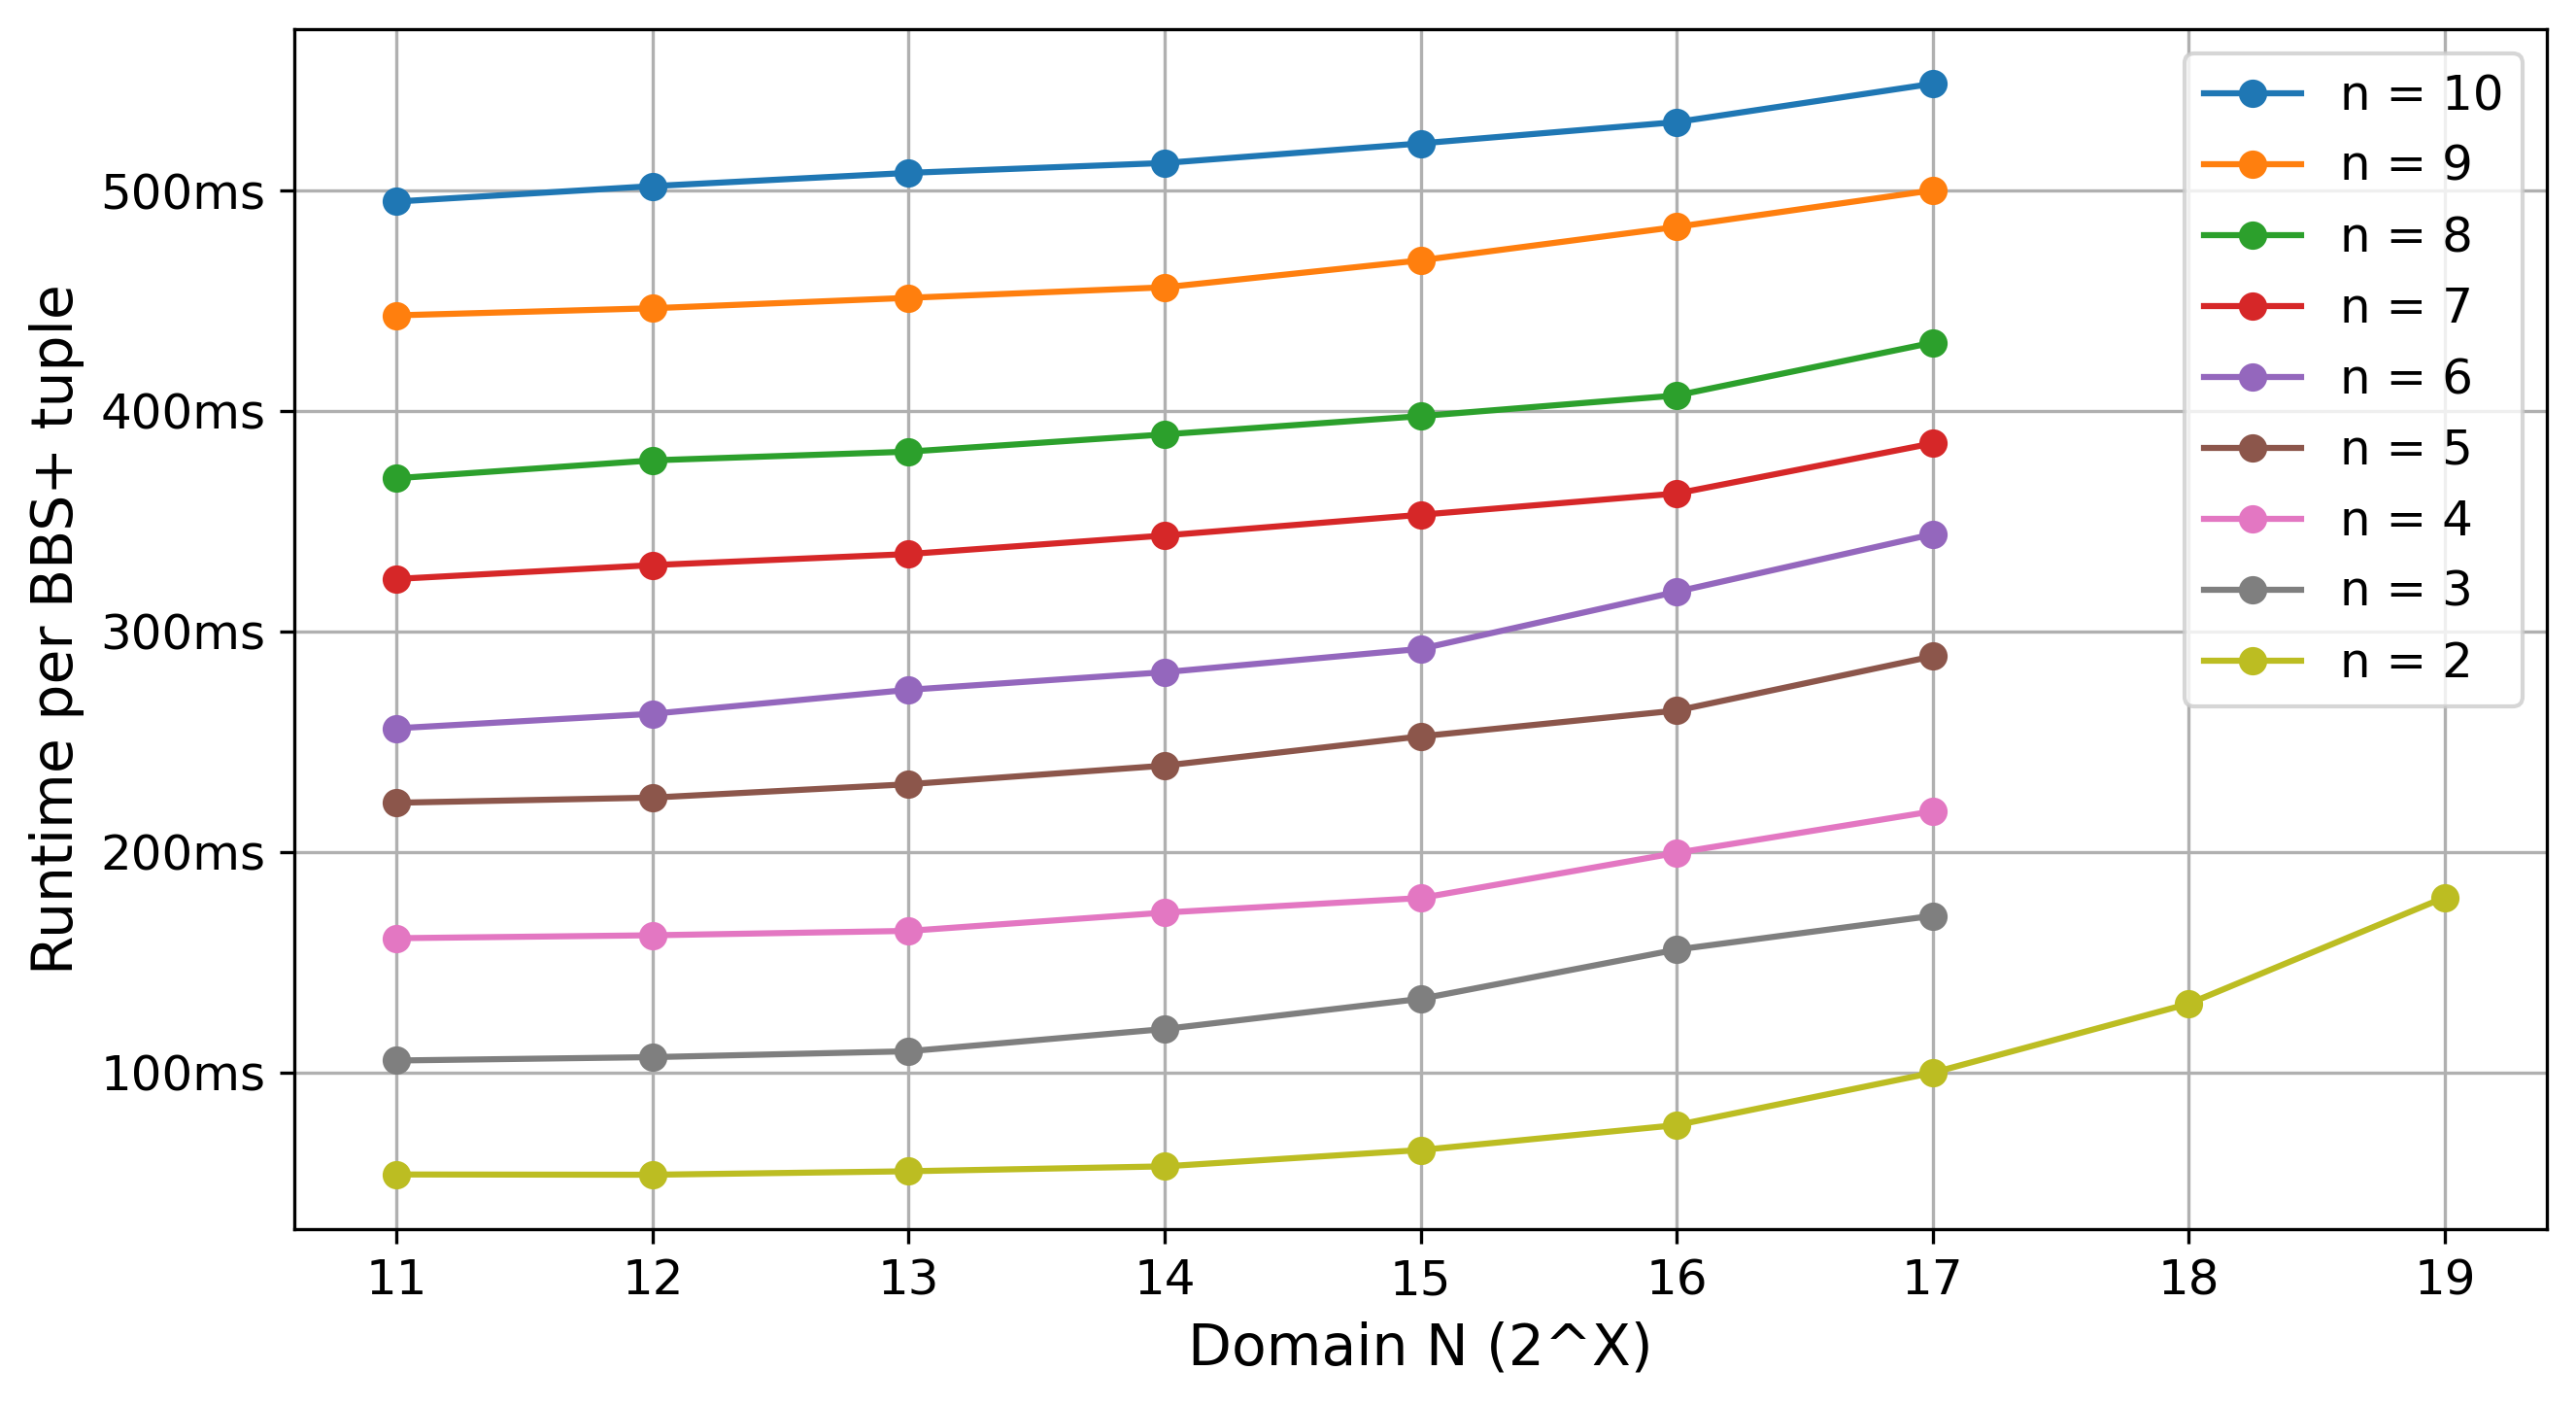
\includegraphics[scale=0.49]{images/plots/bbs_pcg_NoutofN.png}
    \caption{$n$-out-of-$n$ BBS+ PCG expansion over $N$}
    \label{fig:BBSnoutofn}
\end{figure}

\subsection{$t$-out-of-$n$}
\label{subsec:toutofnEval}
We evaluate our implementation of the $t$-out-of-$n$ setting for $t = 2$, parties $n\in \{3, ..., 10\}$ and domains $N\in \{2^{11}, ...,2^{18}\}$ in Figure \ref{fig:BBSnoutofn}. Notably, $t$ does not influence the runtime as described in Section \ref{subsec:tauoutofnSetting}; therefore, the presented numbers hold for any choice of $t$. Again, we observe that the runtime increases quasilinear for domain $N$. In contrast to the $n$-out-of-$n$ setting before, the runtime increase over $N$ is notably steeper. This behavior derives from the construction now needing to deal with more ring elements, leading to more frequent use of FFT. Since FFT is used more frequently, the primitive has a higher (non-linear) impact on the total runtime, resulting in a stronger runtime increase over $N$.
\\\\
\textbf{Comparison to $n$-out-of-$n$.} Directly comparing runtimes, we find the $t$-out-of-$n$ implementation takes roughly 37\% longer for $N=2^{17}$ and $n=3$, with similar overhead existing for other values of $n$. This confirms that the presented adaption for realizing the $t$-out-of-$n$ setting while introducing some overhead remains computationally manageable.
\\\\
\textbf{Introducing Overhead to the Online Phase.} We observe that one major drawback of the $t$-out-of-$n$ approach for Construction \ref{construction:PCGforBBS+} is that we cannot split the ring elements during pre-processing, as the signer set is needed to combine the ring elements accordingly before evaluating them on a specific root of unity. This forces us to perform these operations during the online phase of the threshold BBS+ scheme. Although the amount of ring element evaluations is fixed (to 5), the degree of their polynomial representation is determined by $N$. This implies that choosing larger domains $N$ for the PCG in the offline phase introduces an increasing overhead during the online signing phase. This increase can be quantified as five degree-$N$ polynomial evaluations, therefore by recalling numbers from Figure \ref{fig:polyEvalBench}, the overhead for $N=2^{10}$ amounts to $0.3$ms and $N=2^{18}$ to $18.8$ms. Since the points at which the polynomials need to be evaluated are known in advance, there may be room for improvement since exponentiations could be pre-calculated. In any case, some overhead remains at this stage. We decide to leave this potential optimization as future work.

\begin{figure}[t]
    \centering
    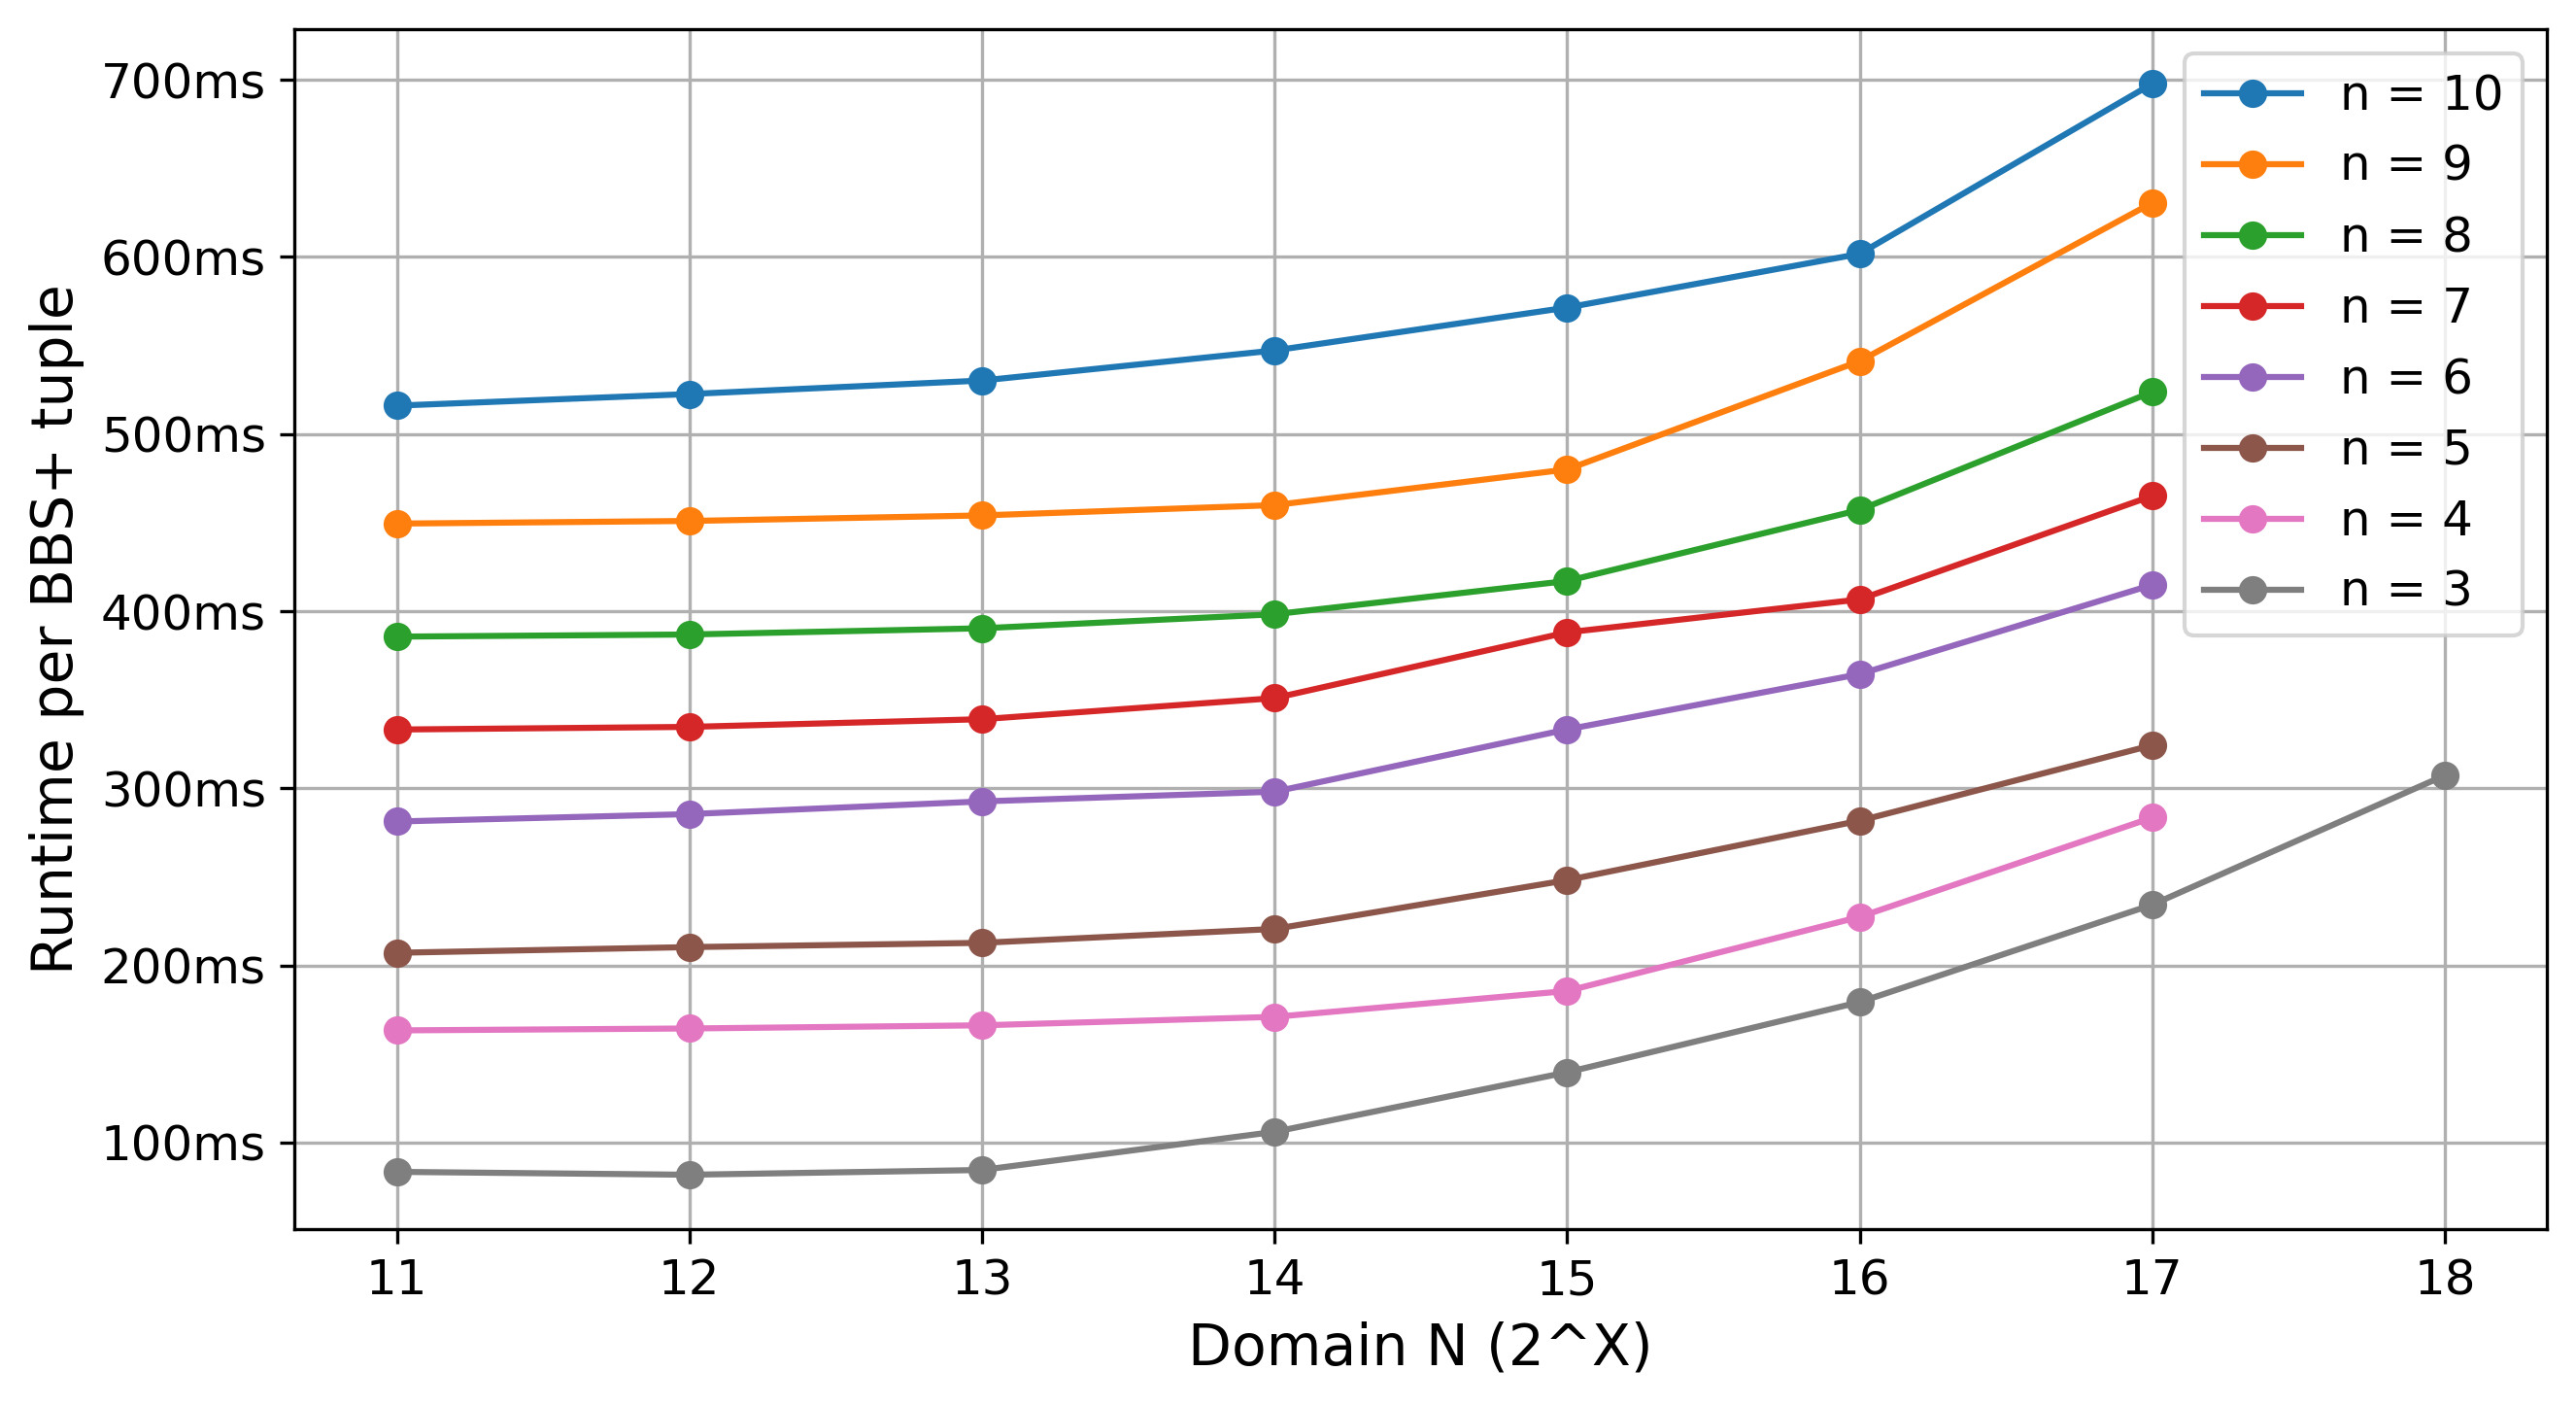
\includegraphics[scale=0.49]{images/plots/bbs_pcg_TAUoutofN.png}
    \caption{$2$-out-of-$n$ BBS+ PCG expansion over $N$}
    \label{fig:BBStauoutofn}
\end{figure}

\subsection{Identifying Bottlenecks}
\label{subsec:bbspPcgBottlenecks}
Recall that in the PCG for (V)OLE, generating ring elements using FFT was the primary performance bottleneck (cf. Figure \ref{fig:runtimeAllocationComparision}), especially for large domains. However, let us analyze how this changes within the context of the BBS+ PCG. Figure \ref{fig:runtimeAllocationComparision} breaks down the construction's runtime for different party counts ($n$) on $N=2^{17}$.
\\\\
In the $t$-out-of-$n$ setting, the proportion of time spent on full domain evaluations versus ring element generation remains roughly constant. This is because as $n$ becomes larger, more full domain evaluations are needed for each of which additional ring elements need to be created. Therefore, the runtime increases similarly for both building blocks, resulting in an allocation that remains close to constant. Interestingly, in the $n$-out-of-$n$ setting, ring element generation becomes less dominant. This trend is expected as the number of ring elements stays fixed while full domain evaluations increase with $n$. Surprisingly, in contrast to FFT being the main cost within the PCG for (V)OLE, our analysis reveals that full domain evaluations of DSPFs represent the primary bottleneck in the PCG for BBS+ Tuples. Therefore, further optimizing this building block would significantly improve the overall performance.
\\\\
\textbf{Comparison to \cite{abram2022low}.}
For evaluating the overall efficiency gains introduced by our practical considerations, we compare our runtimes with the Rust implementation\footnote{\url{https://github.com/ZenGo-X/silent-ecdsa}} of a $n$-out-of-$n$ PCG for threshold ECDSA proposed by Abram et al. in \cite{abram2022low}. Since our construction is derived from theirs, the PCGs are very similar. The main difference is that their PCG incorporates only one OLE and one VOLE correlation, while ours incorporates two OLE and one VOLE. Similar to our implementation, the DSPF building block is parallelized and operates on Boyle et al.'s tree-based approach \cite{boyle2016function}. Therefore, we argue that comparing their implementation to ours is meaningful, although we want to emphasize that Rust generally offers a performance advantage compared to Go in most scenarios\footnote{\url{https://benchmarksgame-team.pages.debian.net/benchmarksgame/fastest/rust-go.html}}. For technical reasons, their selection for the PCG's domain $N$ is not a power of two, but from a given set of optimized values that we adhere to. For a fair comparison, we run their implementation on our test bench and find that for the $2$-out-of-$2$ setting, the PCG requires per pre-signature $247.79$ms for $N=14304$ and $871.83$ms for $N=94019$. These runtimes align (proportionately) with their reported numbers. From our measurements (Figure \ref{fig:BBSnoutofn}), we derive that our implementation significantly outperforms theirs by approximately $6$x-$10$x for the same settings despite generating an additional OLE correlation. In particular, our advantage increases for larger $N$. Consequently, we conclude that the careful optimizations concerning the building blocks as presented in Chapter \ref{chapter:ImplementingPCGs} contribute significant performance improvements to the overall runtime of \texttt{Module-LPN} based PCGs as introduced by Boyle et al. \cite{boyle2020efficient}, therefore positively affecting their practicality. 

\begin{figure}[t]
    %\centering
    \hspace{-1em}
    \begin{subfigure}[b]{0.5\textwidth}
        \centering
        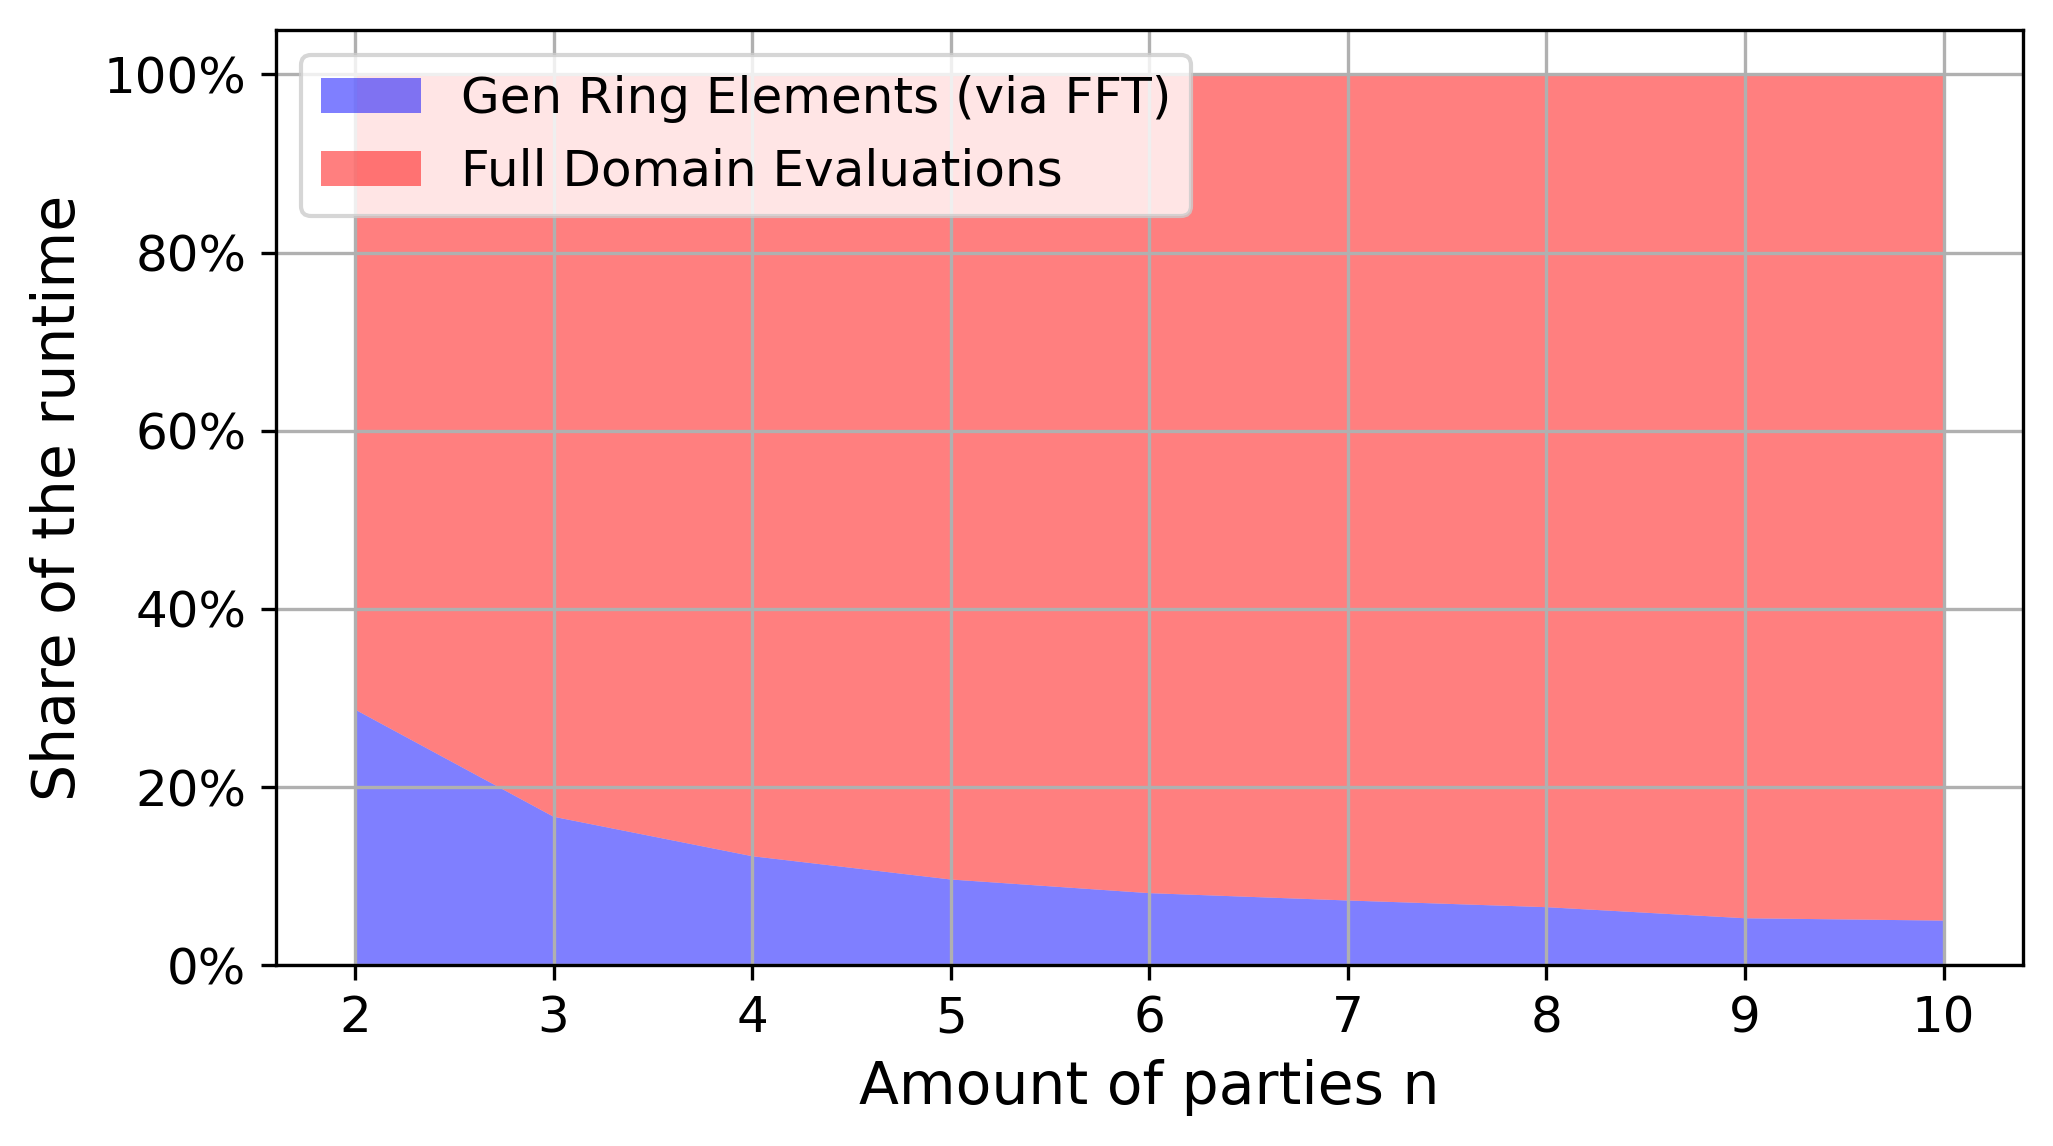
\includegraphics[scale=0.49]{images/plots/bbs_noutofN_percentage_dist.png}
        \caption{$n$-out-of-$n$}
    \end{subfigure}
    \hspace{0em}
    \begin{subfigure}[b]{0.5\textwidth}
        \centering
        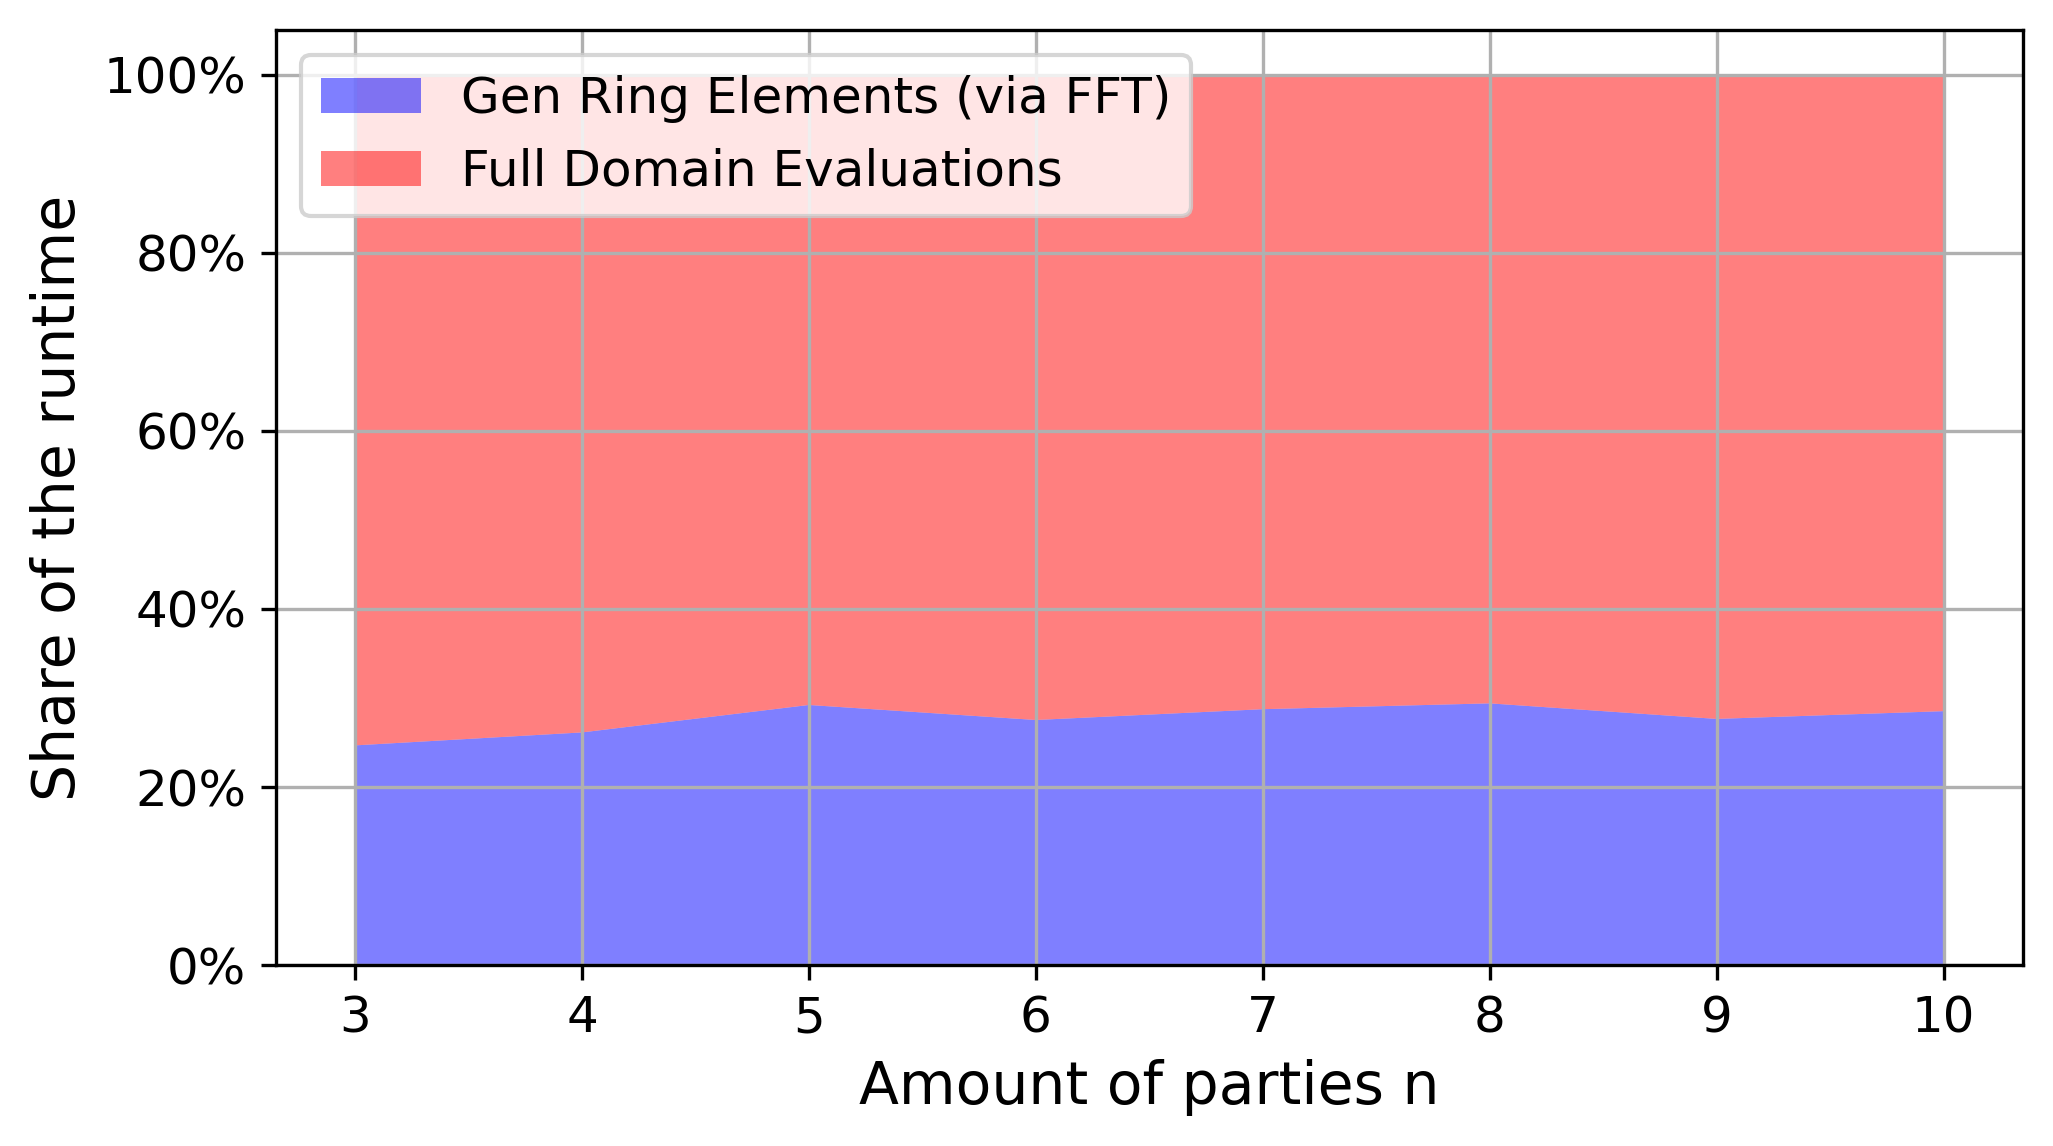
\includegraphics[scale=0.49]{images/plots/bbs_TAUoutofN_percentage_dist.png}
        \caption{$2$-out-of-$n$}
    \end{subfigure}

    \caption{Comparing runtime allocation of $n$-out-of-$n$ with $2$-out-of-$n$ for $N=2^{17}$}
\label{fig:runtimeAllocationComparision}
\end{figure}

\subsection{Implications for Non-
\label{subsec:implNIBBs+}
Interactive Threshold BBS+}
The presented benchmarks show that the implemented PCG, while resource intensive, is practical for the offline pre-processing phase of Faust et al.'s threshold BBS+ scheme \cite{faust2023non}. For the $2$-out-of-$2$ setting, $2^{17}$ signatures can be pre-processed in around $9.5$ hours (under $132$ms per signature), which is certainly practical for some real-world applications, e.g., when pre-processing is performed overnight. Having generated the pre-signatures, Faust et al. \cite{faust2023non} report for the online phase that their implementation of \texttt{ThreshSign} then requires around $0.3$ms per included message $l\in[k]$, with notably no communication needed between the signing parties. Note that communication between the signing parties and the requester must still be accounted for, which makes the server with the highest latency determine the total runtime of the signing protocol. In that regard, Faust et al. compare their online signing phase with an interactive threshold BBS+ protocol by Doerner et al. \cite{doerner2023threshold} that does not employ the preprocessing model. The authors find that the non-interactive approach pays off, especially in the WAN setting, as it achieves between $2$x and $3$x superior runtimes. In the LAN setting, the speedup is increasing linearly over the participating parties, with around $0.5$x for 10 parties to $2$x for 15 parties.
\\\\
While the above evaluation of the online phase holds for the $n$-out-of-$n$ setting, it disregards the overhead the $t$-out-of-$n$ setting introduces. Applying the overhead to the reported numbers reveals that this potentially impacts the protocol's advantage in lower latency settings, dependent on the chosen $N$ in the offline phase. Faust et al. report a runtime of around $8$ms for $k=1$ in the LAN setting, constant for the amount of participating parties. As reported, assuming $N=2^{18}$, additional $18.8$ms need to be accounted for. The overhead can be reduced by making $N$ smaller, but this also results in fewer pre-signatures available. Depending on the amount of participating parties (that drive up the runtime/latency in the interactive scheme) and chosen $N$, the non-interactive approach may loose its advantage in the LAN scenario. Note that this is heavily dependent on the chosen parameters and only effects low-latency settings. The advantage of the non-interactive online phase still holds for high latency settings (like WAN), regardless of the number of participating parties. Therefore, in applications where high latency is a dominant factor, the employed preprocessing model offers a clear advantage over interactive approaches, regardless of the chosen threshold.